\section{DNS theory}

\subsection{The data contained in name servers}


Name servers manage two kinds of data:

\begin{enumerate}
\item The first kind of data held in sets called \Cola{zones}; each zone is the
  complete database for a particular ``pruned'' subtree of the domain space.
  This data is called \Cola{authoritative}. \colz{A name server periodically
    checks to make sure that its zones are up to date, and if not, obtains a new
    copy of updated zones from \cola{master files stored locally} or in
    \cola{another name server}.
  }
\item The second kind of data is \cola{cached data} which was acquired by a
  local resolver.
\end{enumerate}

Depending on its capabilities, a name server could be a standalone program on a
dedicated machine or a process or processes on a large timeshared host. A simple
configuration might be shown in \cref{fig:name-serv-arch}

\begin{figure}[h]
  \centering
  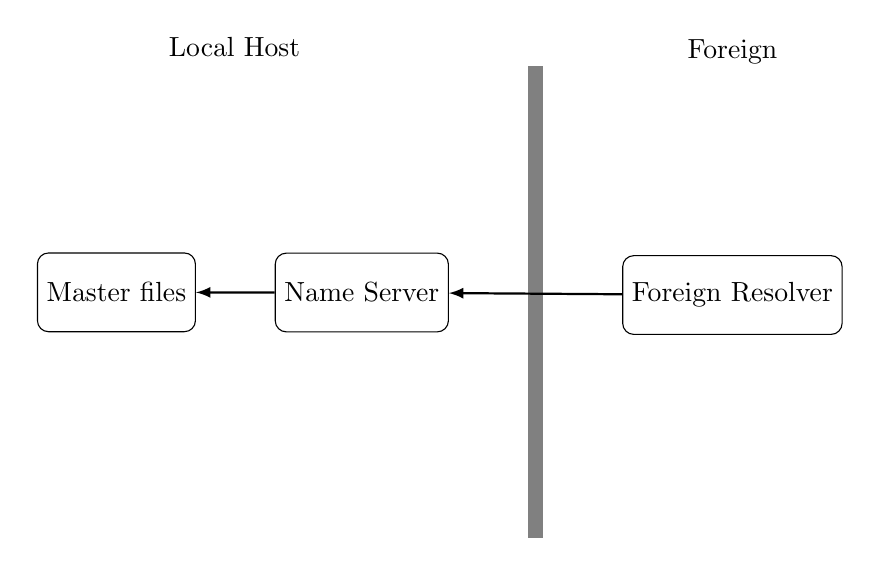
\begin{tikzpicture}
    % \draw[step=1cm,help lines,] (-7.5cm,-5cm) grid +(15cm,10cm);
    \tikzstyle{every node}=[draw=black,anchor=base]
    \matrix[draw=none,column sep=1cm,nodes={minimum size=1cm, rounded corners}] {
      \node[name=mf] {Master files}; &
      \node[name=ns] {Name Server}; &

      \newdimen\x
      \newdimen\y
      \x=3cm
      \y=0.1cm
      \fill[gray] (-\y,-\x) rectangle +(2\y,2\x); &
      \node[name=fr] {Foreign Resolver};\\
    };

    \node[draw=none] at ([shift={(1.5cm,3cm)}]mf) {Local Host};
    \node[draw=none] at ([shift={(0,3cm)}]fr) {Foreign};

    \draw[latex-,thick] (mf) -- (ns);
    \draw[latex-,thick] (ns) -- (fr);
  \end{tikzpicture} 
  \caption{Simple name server architecture}
  \label{fig:name-serv-arch}
\end{figure}

% \clearpage{}

\subsection{The Resource Record (RR) definitions}
\label{sec:rr-defs}

\subsubsection{Format}

All Resource Record (RR) have the same top level format shown in
\cref{tab:rr-format}. The numbers are all big-endien. (the ``internet-endien'')

\newcolumntype{s}{>{\hsize=.2\hsize}X}
\newcolumntype{c}{>{\hsize=.2\hsize \centering\arraybackslash}X}
\begin{table}[h]
  \centering
  \begin{tabularx}{0.8\linewidth}{scX}
    Field& Length (word = 2 bytes) & Description \\[2pt]
    \hline
    \texttt{Name} & 4 & The name of owner, i.e. the node to which this RR pertains. \\[1pt]
    \texttt{Type} & 1 & The RR \texttt{TYPE} code. \\[1pt]
    \texttt{Class} & 1 & The RR \texttt{CLASS} code.\\[1pt]
    \texttt{TLL} & 2 & \texttt{int32} that specifies the time interval that the
                       resource record may be cached before the source of the
                       information should again be consulted. \colz{Zero
                       values are interpreted to mean that the RR can only be
                       used for the transaction in progress, and should not be
                       cached. For example,  \cola{SOA records} are always distributed
                       with a zero TTL to prohibit caching. Zero values can also
                       be used for very volatile data.
                       } \\[1pt]
   \texttt{RDLENGTH} & 2 & \texttt{uint16} that specifies the length in octets
                           of \texttt{RDATA} field. \\[1pt]
         \texttt{RDATA} & variable & The string that describes the resource.
  \end{tabularx}
  \caption{RR top level format}
  \label{tab:rr-format}
\end{table}

\FloatBarrier                   % \usepackage{placeins}

\subsubsection{\texttt{TYPE} values}
Following \texttt{TYPE} fields are available (\cref{tab:rr-types}):
\label{sec:rr-types}
\begin{table}[h]
  \centering
  \begin{tabularx}{0.8\linewidth}{scX}
    TYPE& value & meaning \\[2pt]
    \hline
    \texttt{A} & 1 & a host address \\
    \texttt{NS} & 2 & an authoritative name server \\
    \texttt{CNAME} & 5 & the canonical name for an alias \\
    \texttt{SOA} & 6 & marks the start of a zone of authority \\
    \texttt{WKS} & 11 & a well known service description \\
    \texttt{PTR} & 12 & a domain name pointer \\
    \texttt{HINFO} & 13 & host information \\
    \texttt{MINFO} & 14 & mailbox or mail list information \\
    \texttt{MX} & 15 & mail exchange \\
    \texttt{TXT} & 16 & text strings \\

    \texttt{AAAA} & 28 &  a host address (IPv6) \cola{[RFC3596]}\\
    \texttt{CAA} & 257 &  Certification Authority Authorization: constrains
                         acceptable CAs for a domain. \cola{[RFC6844]}\\
    \texttt{CDS} & 59 & Child copy of DS record \cola{[RFC7344]}
  \end{tabularx}
  \caption{Defined \texttt{TYPE} values}
  \label{tab:rr-types}
\end{table}

\cSay{
  \colz{
    You may have noticed that some of the values are missing, e.g. \texttt{3,
      4}. Those are either obsolete or experimental.
  }
}

\texttt{TYPE} values are in fact subset of \texttt{QTYPE} values. \texttt{QTYPE}
values that are not \texttt{TYPE} values are shown in \cref{tab:qtypes}.

\begin{table}[h]
  \centering
  \begin{tabularx}{0.8\linewidth}{scX}
    QTYPE& value & meaning \\[2pt]
    \hline
    \texttt{AXFR} & 252 & A request for a transfer of an entire zone \\
    \texttt{MAILB} & 253 & A request for mailbox-related records \\
    \texttt{*} & 255 & A request for all records \\
  \end{tabularx}
  \caption{Defined \texttt{QTYPE} values}
  \label{tab:qtypes}
\end{table}

\subsubsection{\texttt{CLASS} values}

You just need to remember one value: \texttt{IN} (value=1) which stands for
``internet''. Occasionally you might also see \texttt{CH} (value=3) which stands
for ``chaos'', it is usually used to determine some versions.


\subsubsection{\texttt{A RDATA} format}
\texttt{A} RDATA is just a normal IPv4 address, such as \texttt{1.2.3.4.}

\subsubsection{\texttt{NS RDATA} format}
NS record is just a domain name.

NS records cause both
\begin{itemize}
\item the usual additional section processing to locate a type \texttt{A} record
\item and, when used in a referral, a special search of the zone in which they
  reside for glue information.
\end{itemize}


\subsubsection{\texttt{CNAME RDATA} format}

\texttt{CNAME} RDATA just contains a \cola{domain name}, which is represented as
a series of labels, and terminated by a label with zero length.

\subsubsection{\texttt{SOA RDATA} format}

\texttt{SOA} RDATA has the following format (\cref{tab:soa-rdata}).

\begin{table}[h]
  \centering
  \begin{tabularx}{0.8\linewidth}{sX}
    Field & Description \\[2pt]
    \hline
    \texttt{MNAME} & \colz{
                     The \cola{\texttt{<domain-name>}} of the name server that was the original of data for this zone.
                     }\\
    \texttt{RNAME} & \colz{Admin's email} \\
    \texttt{SERIAL} & \colz{
                      \texttt{uint32} \cola{version number} of the original copy of the zone.
                      }\\
    \texttt{REFRESH} & \colz{
                       \texttt{uint32} time interval before the zone should be
                       \colZ{refreshed}.
                       }\\
    \texttt{RETRY} & \colz{
                      \texttt{uint32} Retry-time for failed \texttt{REFRESH}
                     }\\
    \texttt{EXPIRE} & \colz{
                      Expire-time
                      }\\
    \texttt{MINIMUM} & \colz{
                       \texttt{uint32}
                       Minimum allowable TTL value exportable from this zone.
                        }\\
  \end{tabularx}
  \caption{SOA RDATA format}
  \label{tab:soa-rdata}
\end{table}

All times are in units of seconds.

\subsection{Message}

All DNS messages have the same top level format shown in \cref{tab:msg-format}.

\begin{table}[h]
  \centering
  \begin{tabularx}{0.8\linewidth}{sX}
    Field & Description \\[2pt]
    \hline
    \texttt{Header} & A fixed format header. \\
    \texttt{Question} & the question for the name server. \\
    \texttt{Answer} & RRs answering the question. \\
    \texttt{Authority} & RRs pointing toward an authority. \\
    \texttt{Additional} & RRs holding additional information. \\
  \end{tabularx}
  \caption{The DNS message format}
  \label{tab:msg-format}
\end{table}

\subsubsection{Header}

The header contains the following fields (\cref{tab:msg-header,tab:msg-header2}).

\begin{table}[h]
  \centering
  \begin{tabularx}{0.8\linewidth}{scX}
    field & size (bits) & meaning \\[2pt]
    \hline
    \texttt{ID} & 16 & Id assigned by the \cola{program that
                       generates the query}. \colz{
                        This id is copied the corresponding reply and
                       can be used by the \colZ{requester} to match up replies
                       to outstanding queries.
                       } \\
    \texttt{QR} & 1 & \colz{
                      A one bit field that specifies whether this message is a
                      \colZ{query (0), or a response (1).}} \\
    \texttt{OPCODE} & 4 & \colz{
                          the kind of query. It can be
                          \begin{align*}
                            0 &\quad \Rightarrow \text{a standard query (QUERY)}\\
                            1 &\quad \Rightarrow \text{an inverse query (IQUERY)}\\
                            2 &\quad \Rightarrow \text{a server status request}\\
                            3-15 &\quad \Rightarrow \text{reserved for future use}
                          \end{align*}
                                   } \\
    \texttt{AA} & 1 & \colz{Authoritative Answer. Only valid in responses. It
                      means that \colZ{the responding name server is an
                      authority for the domain name in question section.}
                      }
    \\
  \end{tabularx}
  \caption{The DNS message header format}
  \label{tab:msg-header}
\end{table}

\dSay{Oh, so it's like we have to keep asking until this bit is set?}

\cSay{
  \colz{
    No. It's just a flag that tells you whether the
    responding name server is an authority for the domain name in question
    section.
  }
}

\begin{table}[h]
  \centering
  \begin{tabularx}{0.8\linewidth}{scX}
    field & size (bits) & meaning \\[2pt]
    \hline
    \texttt{TC} & 1 & \colz{This message is truncated}\\
    \texttt{RD} & 1 & \colz{Recursion Desired.

                      If \colZ{RD} is set, it
                      directs the name server to pursue the query recursively.
                      \colZ{Recursive query support is optional.}
                      } \\
    \texttt{RA} & 1 & \colz{Recursion Available in the name server.}\\
    \texttt{Z} & 3 & \colz{Reserved for future use. Must be zero in all queries
                     and responses.}\\
    \texttt{RCODE} & 4 & \colz{Response code. It can be
                         \begin{align*}
                           0 &\quad \Rightarrow \text{No error condition}\\
                           1 &\quad \Rightarrow \text{Format error}\\
                           2 &\quad \Rightarrow \text{Server failure}\\
                           3 &\quad \Rightarrow \text{Name error}\\
                           4 &\quad \Rightarrow \text{Not implemented}\\
                           5 &\quad \Rightarrow \text{Refused}
                         \end{align*}
                               } \\
    \texttt{QDCOUNT} & 16 & \colz{an \texttt{uint16} specifying the number of entries in the
                            \colZ{question section}.}\\
    \texttt{ANCOUNT} & 16 & \colz{an \texttt{uint16} specifying the number of
                            RRs in
                            the \colZ{answer section}.}\\
    \texttt{NSCOUNT} & 16 & \colz{an \texttt{uint16} specifying the number of name server
                            RRs in the \colZ{authority records
                            section}.}\\
    \texttt{ARCOUNT} & 16 & \colz{an \texttt{uint16} specifying the number of
                            RRs in the \colZ{additional records section}.}\\
  \end{tabularx}
  \caption{The DNS message header format}
  \label{tab:msg-header2}
\end{table}

\FloatBarrier

\subsubsection{Question}

The question section contains \texttt{QDCOUNT} (usually 1) entries, each is
shown in \cref{tab:msg-question}.

\begin{table}[h]
  \centering
  \begin{tabularx}{0.8\linewidth}{scX}
    field & size (bits) & meaning \\[2pt]
    \hline
    \texttt{QNAME} & variable & \colz{a domain name represented as a sequence of labels,
                                where each label consists of a length octet
                                followed by that number of octets.

                                The domain
                                name terminates with the zero length octet for
                                the null label of the root. Note that this field
                                may be an \cola{odd number of octets} (i.e., not
                                \cola{word aligned}).
                                } \\
    \texttt{QTYPE} & 16 & \colz{a \texttt{TYPE} field.}\\
    \texttt{QCLASS} & 16 & \colz{a \texttt{CLASS} field.}\\
  \end{tabularx}
  \caption{The DNS message question format}
  \label{tab:msg-question}
\end{table}

\FloatBarrier
\subsubsection{Answer, Authority, Additional}

The answer, authority, and additional sections all share the same format: a
variable number of \Cola{resource record}, which is shown previously in
\cref{tab:rr-format} as we discussed in \cref{sec:rr-defs}.

\subsection{message compression}
\label{sec:cmpr}

There's a compression mechanism in DNS messages, which uses pointers to avoid
duplicated domain names. But let's skip it for now.

\subsection{Transport}

DNS server uses both UDP (port 53) and TCP (port 53). For UDP the size of a
message is limited to 512 bytes, excluding the IP and UDP headers.

\subsection{Zone files (master files)}
\label{sec:mfile}

If RRs are data, then zone files are the database (in plain text).

\colz{
  The format is a sequence of entries. Each is a single line. (can be extended
  using parentheses). Any combination of tabs and spaces act as a delimiter that
  separates items that make up an entry.

  The end of any line can end with a comment. A comment starts with a ``\texttt{;}''
}

\subsubsection{zone file entries}
\label{sec:zone-entries}

The following entries are available:

\begin{enumerate}
\item \texttt{\cola{\$ORIGIN}  \colc{<domain-name>}} : \colz{resets the \colZ{current
    origin} for \colZ{relative domain names} to the stated name.
  }
\item \texttt{\cola{\$INCLUDE} <file-name> \colc{[<domain-name>]}} : \colz{inserts
    the named file into the current file. If the domain name is present, it
    specifies its \cola{\texttt{\$ORIGIN}}. Note that this entry never change
    the relative origin of the parent file.
  }
\item \texttt{\colc{[<domain-name>]}<rr>} : \colz{
    an actual RR record. If the domain name is missing, then the RR belongs to
    the last stated owner.
  }
\end{enumerate}

Blank lines, with or without comments, are allowed.

\subsubsection{Format of RR}
\label{sec:rr-format}

Each \texttt{<rr>} has the following forms:

\begin{center}
  \ttfamily
 \cola{[<class>]} \colb{[<TTL>]} \cola{<type>} <RDATA>
\end{center}

Where the order of \texttt{\cola{<class>}} and \texttt{\colb{<TTL>}} can varies.

\texttt{\colb{<TTL>}} is a decimal integer. If either \texttt{\cola{<class>}} or
\texttt{\colb{<TTL>}} is missing, the last value stated is used.

\texttt{\colc{[<domain-name>]}} are expressed as a sequence of character strings
separated by dots. \colz{Domain names that end in a dot are called \cola{fully
    qualified domain names} (FQDNs). Domain names that do not end in a dot are
  called \cola{relative domain names} (RDNs). In that case, the actual domain
  name is the concatenation of the RDN and the \texttt{\cola{\$ORIGIN}}.
}

\subsubsection{Character string}
\label{sec:char-string}
Character string is expressed in two ways:

\begin{enumerate}
\item a contiguous set of characters without spaces. For example, \texttt{aaa}
\item a string quoted by double quotes. For example, \texttt{"aaa bbb"}
\end{enumerate}

\subsubsection{Special characters}

Some characters are special, as shown in \cref{tab:zone-spec-char}.

\begin{table}
  \centering
  \begin{tabularx}{0.8\linewidth}{sX}
    \texttt{@} &  A free standing \texttt{@} denote the \cola{\texttt{\$ORIGIN}}.\\
    \verb|\X| &  Char escape, e.g. \verb|\"| to mean \texttt{"}\\ \\
    \verb|\DDD| &  Octal escape, e.g. \verb|\100| to mean \texttt{@}\\ \\
  \end{tabularx}
  \caption{Special characters in zone file}
  \label{tab:zone-spec-char}
\end{table}

\subsubsection{Rules}
\label{sec:zone-file-rules}

In addition to the grammar rules, following rules are also applied:

\begin{enumerate}
\item \colz{All RRs in the file should have the same \cola{\texttt{<class>}}}
\item Exactly one \texttt{SOA RR} \colz{should be present at the top of the
    zone.}
\item \colz{If delegations are present and glue information is required, it
    should be present. (??)
  }
\item \colz{Info present outside of the authoritative nodes in the zone should
    be glue information, rather than the result of an origin or similar error.}
\end{enumerate}
